%%%%%%%%%%%%%%%%
\section{Control Approach}

\begin{frame}{Control Approach}{}
    \begin{figure}[H]
        \centering
        \includegraphics[width=.6\linewidth]{figures/controllerDiagram2}
    \end{figure}
\end{frame}

%%%%%%%%%%%%%%%%
\section{Sensor Fusion}

\begin{frame}{Sensor Fusion}{Structure}
	\begin{itemize}

		\item Fuses GPS and IMU data
		\item Achieved using a Kalman filter
		\item Sensor fusion contains
			\begin{itemize}
		\item Attitude
		\item Position
			\end{itemize}
	\end{itemize}

\end{frame}
\begin{frame}{Sensor Fusion}{Signal Model}
	\begin{gather*}
    \vec{x}_\mathrm{KF}(k+1) = \vec{A}_\mathrm{KF}\vec{x}_\mathrm{KF}(k) + \vec{B}_\mathrm{KF} \vec{u}(k) + \vec{w}_\mathrm{KF}(k)  \nonumber \\
    \vec{y}_\mathrm{KF}(k+1) = \vec{C}_\mathrm{KF} \vec{x}_\mathrm{KF}(k+1) + \vec{v}_\mathrm{KF}(k+1)  \nonumber
    \end{gather*}
    \begin{figure}[H]
        \centering
        \includegraphics[width=.7\linewidth]{figures/signalModel}
    \end{figure}
	\begin{itemize}
		\item w(k) and v(k) are assumed white Gaussian
		\item Matrices $\vec{Q}_\mathrm{KF}$ and $\vec{R}_\mathrm{KF}$ are the respective covariance matrices
	\end{itemize}

\end{frame}

\begin{frame}{Sensor Fusion}{Signal Model - State and Measurement Vectors}
    \begin{flalign}
        \vec{u} = 
        \begin{bmatrix}
        F_1 & F_2
        \end{bmatrix}^\mathrm{T}  \nonumber
    \end{flalign}
\begin{itemize}
    \item Attitude
    \begin{gather*}
        \vec{x}_\mathrm{att} = 
        \begin{bmatrix}
        \phi & \theta & \psi & \dot{\phi} & \dot{\theta} & \dot{\psi} & \ddot{\phi} & \ddot{\theta} & \ddot{\psi}
        \end{bmatrix}^\mathrm{T}  \nonumber \\
        \vec{y}_\mathrm{att} =
        \begin{bmatrix}
        \phi_\mathrm{acc} & \theta_\mathrm{acc} & \psi_\mathrm{mag} & \dot{\phi}_\mathrm{gyro} & \dot{\theta}_\mathrm{gyro} & \dot{\psi}_\mathrm{gyro}
        \end{bmatrix}^\mathrm{T} \nonumber
    \end{gather*}
	\item Position
    \begin{gather*}
        \vec{x}_\mathrm{pos} =
        \begin{bmatrix}
        x_\mathrm{n} & y_\mathrm{n} & \dot{x}_\mathrm{b} & \dot{y}_\mathrm{b} & \ddot{x}_\mathrm{b} & \ddot{y}_\mathrm{b}
        \end{bmatrix}^\mathrm{T} \nonumber \\
        \vec{y}_\mathrm{pos} =
        \begin{bmatrix}
        x_\mathrm{n,GPS} & y_\mathrm{n,GPS} & \ddot{x}_\mathrm{b,acc} & \ddot{y}_\mathrm{b,acc}
        \end{bmatrix}^\mathrm{T} \nonumber
    \end{gather*}
    \end{itemize}
\end{frame}


\begin{frame}{Sensor Fusion}{Kalman Filter}

	\begin{itemize}
		\item Step 0: Initialization
        \begin{flalign}
        	\hat{\vec{x}}_\mathrm{KF}(0|0) &= \vec{0} \nonumber\\
        	\vec{P}_\mathrm{KF}(0|0) &= \vec{Q}_\mathrm{KF}\nonumber
        \end{flalign}
		\item Step 1: Prediction
		\item Step 2: Update
   	\end{itemize}
\end{frame}


\begin{frame}{Sensor Fusion}{Kalman Filter}
	\begin{itemize}
		\item Step 0: Initialization
		\item Step 1: Prediction
        {\footnotesize
        \begin{flalign}
            \hat{\vec{x}}_\mathrm{KF}(k+1|k) &= \vec{A}_\mathrm{KF} \hat{\vec{x}}_\mathrm{KF}(k|k) + \vec{B}_\mathrm{KF} \vec{u}(k) \nonumber\\
            \vec{P}(k+1|k) &= \vec{A}_\mathrm{KF} \vec{P}(k|k) \vec{A}_\mathrm{KF}^\mathrm{T} + \vec{Q}_\mathrm{KF} \nonumber
        \end{flalign}}
	 	\item Step 2: Update
         {\footnotesize
        \begin{gather*}
            \hat{\vec{x}}_\mathrm{KF}(k+1|k+1) = \hat{\vec{x}}_\mathrm{KF}(k+1|k) +  \vec{K}(k+1) \left[ \vec{y}_\mathrm{KF}(k+1) - \vec{C}_\mathrm{KF}  \hat{\vec{x}}_\mathrm{KF}(k+1|k) \right] \nonumber\\
            \vec{P}(k+1|k+1) = \left[ \vec{I} - \vec{K}(k+1) \vec{C}_\mathrm{KF}^\mathrm{T} \right] \vec{P}(k+1|k)\nonumber
        \end{gather*}}
	\end{itemize}
\end{frame}

\begin{frame}{Sensor Fusion}{Kalman Filter}
    \begin{figure}[H]
        \centering
        \includegraphics[width=.95\linewidth]{figures/kalmanFilter}
    \end{figure}
\end{frame}

\begin{frame}{Sensor Fusion}{Attitude Kalman Filter}
    \begin{figure}[H]
        \centering
        \includegraphics[width=0.6\linewidth]{figures/sim_yaw}
    \end{figure}
\end{frame}

\begin{frame}{Sensor Fusion}{Position Kalman Filter}
    \begin{minipage}{0.45\linewidth}
        \begin{figure}[H]
            \centering
            \includegraphics[width=1\linewidth]{figures/sim_xbdot}
        \end{figure}        
    \end{minipage}\hfill      
    \begin{minipage}{0.45\linewidth}
        \begin{figure}[H]
            \centering
            \includegraphics[width=1\linewidth]{figures/sim_xnyn}
        \end{figure}                
    \end{minipage}\hfill \\
\end{frame}

